% HealthNest - project report in IEEE conference format (IEEEtran).
% Compile on Overleaf: upload the zip, set the main document to healthnest_ieee.tex, compiler pdfLaTeX.
% Tables in tables/ and figures in figures/ are generated by report/make_figures.py from the saved
% evaluation results in eval/model_comparison/, so the numbers here match the code.
\documentclass[conference]{IEEEtran}
\IEEEoverridecommandlockouts
\usepackage{cite}
\usepackage{amsmath,amssymb}
\usepackage{graphicx}
\usepackage{booktabs}
\usepackage{array}
\usepackage{url}
\usepackage{xcolor}

\begin{document}

\title{HealthNest: A Verifiable, Multilingual Retrieval-Augmented Health Question-Answering System with Link Analysis, Relevance Feedback and Private Patient Memory}

% TODO: check names, add roll numbers / department / e-mail as your course requires.
\author{\IEEEauthorblockN{Preksha Chavan, Aaditya Kharkia, Aditya Chauhan}
\IEEEauthorblockA{\textit{Department of Computer Science and Engineering} \\
\textit{Shiv Nadar University}\\
Greater Noida, India}}

\maketitle

\begin{abstract}
Health information websites usually serve static pages, and chat-based assistants built on large language models (LLMs) can state unsupported or wrong facts. Retrieval-augmented generation (RAG) reduces this risk by answering from retrieved documents, but typical RAG systems answer every question, work only in English and hide how evidence was chosen. We present HealthNest, an evidence-grounded health question-answering system that extends a recent RAG architecture for medical web platforms~\cite{fedallah2026}. HealthNest indexes 70,154 passages from the NIH MedQuAD collection~\cite{abacha2019} with a hand-written inverted index, combines SMART lnc.ltc TF-IDF and multilingual dense retrieval with Reciprocal Rank Fusion~\cite{cormack2009}, re-ranks with PageRank~\cite{page1999} and HITS~\cite{kleinberg1999} over an inferred topic graph, suggests related topics with topic-sensitive PageRank~\cite{haveliwala2002} and refines results with Rocchio relevance feedback~\cite{rocchio1971}. Every generated sentence must cite a passage and is checked by a sentence-level fact checker; the system abstains when evidence is weak, asks permission before searching Wikipedia, and answers questions about a patient's own prescription or lab report verbatim without sending them to an external service. On a test set of 40 health needs written in English, Hinglish and Hindi plus 20 off-topic questions, HealthNest reached a mean nDCG@10 of 0.313 and P@5 of 0.413, refused all 20 off-topic questions (precision 1.000) and answered 97.5\% of English health questions. Simulated relevance feedback raised nDCG@10 on unseen passages from 0.274 to 0.365 ($p<0.001$). A comparison of four embedding models shows that BGE-M3~\cite{chen2024} gives the best overall ranking (nDCG@10 0.384), while the English-only model of~\cite{fedallah2026} performs best in English but almost fails in Hindi (0.038).
\end{abstract}

\begin{IEEEkeywords}
information retrieval, retrieval-augmented generation, medical question answering, PageRank, HITS, Rocchio relevance feedback, Hinglish, abstention
\end{IEEEkeywords}

%====================================================================
\section{Introduction}
%====================================================================
\textbf{Background.} People increasingly look up symptoms, medicines and test results online before, or instead of, seeing a doctor. General-purpose chat assistants answer fluently but can state facts that no source supports, which is especially risky for doses and warning signs. Retrieval-augmented generation (RAG)~\cite{lewis2020} grounds an LLM in documents returned by a retriever, so that answers can be traced to sources.

\textbf{Importance and motivation.} Fedallah and \.{I}nik~\cite{fedallah2026} showed that a low-cost RAG pipeline (all-MiniLM-L6-v2 embeddings, ChromaDB, Llama~3.3 via Groq) can turn a static medical website into a question-answering system, with a RAGAS~\cite{es2024} faithfulness of 0.888 on 50 interactions. Their system, however, (i) uses 56 chunks from one website, (ii) always passes the top five chunks to the LLM with no similarity threshold, (iii) supports English only, and (iv) does not report retrieval quality. The authors themselves list a larger knowledge base and multilingual support as future work. In India many users write health questions in Hinglish (Hindi in Roman script, e.g., \textit{pet dard} for stomach pain) or in Devanagari, and patients often want to ask about their own prescriptions and lab reports, which must stay private.

\textbf{Contributions.}
\begin{enumerate}
  \item A complete, hand-written IR pipeline over 70,154 MedQuAD passages: multi-zone inverted index, SMART lnc.ltc TF-IDF, Okapi BM25, multilingual dense retrieval and Reciprocal Rank Fusion, with Hinglish lexicon expansion.
  \item Link analysis on a corpus without hyperlinks: a topic-mention graph (4,774 topics, 36,791 links) used for PageRank and HITS re-ranking, and topic-sensitive PageRank with a \emph{lift} score for related-topic suggestions.
  \item Rocchio relevance feedback in both the sparse and the dense vector space (``More like this / Not relevant''), plus an evaluated pseudo-relevance variant.
  \item Trust features: sentence-level citations and fact checking, a three-gate abstention rule, permission-based Wikipedia fallback, and a private patient memory that quotes prescription and report lines verbatim and compares lab values only with the range printed on the report.
  \item A trilingual evaluation (English, Hinglish, Hindi) comparing the retriever of~\cite{fedallah2026} with three other embedding models and reporting precision, recall, F1, MRR, nDCG and abstention accuracy.
\end{enumerate}

%====================================================================
\section{Literature Review}
%====================================================================
\textbf{RAG for medicine.} Lewis \textit{et al.}~\cite{lewis2020} introduced RAG, combining a dense retriever with a generator so that knowledge comes from an index rather than model weights. Fedallah and \.{I}nik~\cite{fedallah2026}, the base of this work, integrated RAG into a Laravel/React medical website and measured faithfulness with RAGAS~\cite{es2024}, an LLM-judged metric of whether an answer is supported by its context. Xiong \textit{et al.}~\cite{xiong2024} benchmarked medical RAG (MIRAGE) with several retrievers and corpora and found that BM25 and the biomedical retriever MedCPT were the strongest single retrievers, and that fusing them with Reciprocal Rank Fusion was a good choice for PubMed.

\textbf{Medical question-answer data.} Ben Abacha and Demner-Fushman~\cite{abacha2019} built MedQuAD, 47,457 question-answer pairs from trusted NIH websites, and answered consumer questions by retrieving and matching similar questions. HealthNest uses the publicly released MedQuAD answers as its corpus.

\textbf{Lexical and dense retrieval.} The probabilistic relevance framework and BM25~\cite{robertson2009} remain strong lexical baselines; the vector space model with SMART weighting is described in~\cite{manning2008}. Reimers and Gurevych~\cite{reimers2020} distilled English sentence embeddings into multilingual models covering 50+ languages, including Hindi. MedCPT~\cite{jin2023} is a biomedical retriever trained on 255 million PubMed query-article clicks. BGE-M3~\cite{chen2024} provides dense, sparse and multi-vector retrieval in more than 100 languages from one model. Reciprocal Rank Fusion (RRF)~\cite{cormack2009} merges rankings without training and outperformed Condorcet fusion and learned rankers.

\textbf{Link analysis and feedback.} PageRank~\cite{page1999} scores pages by the stationary distribution of a random surfer; HITS~\cite{kleinberg1999} computes query-specific hubs and authorities on a focused subgraph; topic-sensitive PageRank~\cite{haveliwala2002} biases the surfer's restarts towards topics. Rocchio's relevance feedback~\cite{rocchio1971} moves the query vector towards documents marked relevant and away from non-relevant ones.

\textbf{Novelty.} Compared with~\cite{fedallah2026}, HealthNest (a) evaluates retrieval itself with labelled relevance, not only answer faithfulness; (b) refuses to answer when evidence is weak instead of always using the top five chunks; (c) supports Hinglish and Hindi; (d) adds link analysis and relevance feedback to a RAG system; and (e) handles personal medical documents with a privacy-preserving, verbatim design. To our knowledge, applying PageRank, HITS and topic-sensitive PageRank to an \emph{inferred} topic-mention graph of a consumer-health RAG corpus, and evaluating them across English, Hinglish and Hindi, has not been reported in the works above.

%====================================================================
\section{Objective}
%====================================================================
The objectives were to: (1) build a health question-answering system whose every answer sentence is traceable to a retrieved passage; (2) implement the core IR algorithms of the course by hand (inverted index, TF-IDF, BM25, fusion, PageRank, HITS, Rocchio) and measure their effect; (3) answer only when evidence is sufficient and otherwise abstain; (4) serve English, Hinglish and Hindi users; (5) let patients ask about their own prescriptions and lab reports without the documents leaving the computer; and (6) compare the retriever of the base paper~\cite{fedallah2026} with alternatives on the same data.

%====================================================================
\section{Proposed Model}
%====================================================================
Fig.~\ref{fig:pipeline} shows the pipeline. A question first passes a safety guard (emergency keywords add a banner; self-harm keywords return helpline information and skip retrieval). If the question refers to the patient's own documents, matching lines are quoted verbatim from the uploaded PDF; general knowledge about the medicines or tests is then retrieved from the corpus, and all generation runs locally. Otherwise the question is normalised and expanded with a 113-entry Hinglish lexicon, sparse and dense retrieval run in parallel and are fused with RRF, and the fused list is re-ranked with PageRank and HITS. An abstention step decides whether the evidence is strong enough. If it is, an LLM (Groq, a local Ollama model, or an offline extractive generator) writes an answer in which every sentence ends with a citation, and a fact checker labels each sentence. If it is not, the system says ``I don't know'' and offers a Wikipedia search, which runs only after the user approves the exact words. The answer page shows citations, support badges, related topics and an IR inspector; ``More like this / Not relevant'' marks trigger a Rocchio re-search.

\begin{figure*}[t]
  \centering
  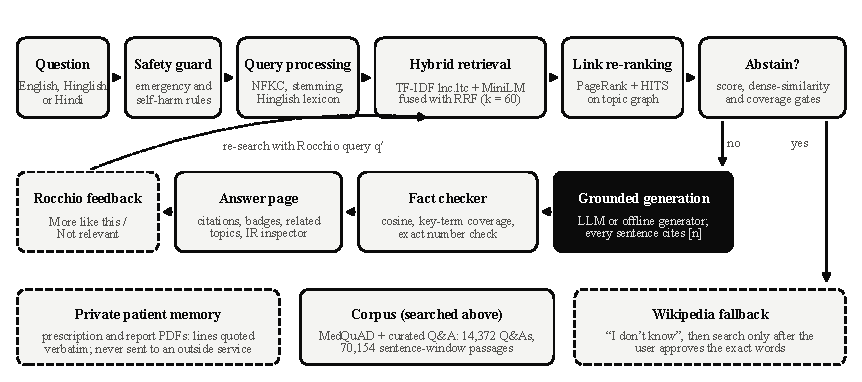
\includegraphics[width=\textwidth]{figures/fig_pipeline.pdf}
  \caption{HealthNest architecture. Solid boxes form the main question-answering path; dashed boxes are optional paths (relevance feedback, private patient memory, permission-based Wikipedia search).}
  \label{fig:pipeline}
\end{figure*}

%====================================================================
\section{Methodology}
%====================================================================
\subsection{Corpus, chunking and indexing}
Three CSV files are read with automatic column detection, empty rows are dropped and exact duplicate questions are removed. Each answer is split into sentence windows of at most 80 words with a one-sentence overlap; a passage keeps its question as a title. Text is NFKC-normalised and lower-cased; tokens match \verb|[\w\u0900-\u097F]+| so that Devanagari vowel signs are not split; English and Hinglish stop words are removed and Porter stemming is applied to ASCII tokens. A hand-written inverted index stores postings separately for a title zone and a body zone.

\subsection{Sparse retrieval}
Documents use \textit{lnc} weights and queries \textit{ltc} weights~\cite{manning2008}:
\begin{equation}
w_{t,d} = 1+\log tf_{t,d}, \qquad w_{t,q} = (1+\log tf_{t,q})\,\log\frac{N}{df_t},
\end{equation}
both cosine-normalised. Scores are accumulated term-at-a-time per zone and combined as $s(q,d)=0.6\cos_{\text{title}}+0.4\cos_{\text{body}}$. BM25~\cite{robertson2009} is also implemented with $k_1=1.2$, $b=0.75$:
\begin{equation}
\text{BM25}(q,d)=\sum_{t\in q}\log\!\Big(\frac{N-df_t+0.5}{df_t+0.5}+1\Big)\frac{tf_{t,d}(k_1+1)}{tf_{t,d}+k_1\big(1-b+b\frac{|d|}{\text{avgdl}}\big)}.
\end{equation}

\subsection{Dense retrieval and fusion}
Passages (title plus text) are embedded with the multilingual model of~\cite{reimers2020} and L2-normalised, so cosine similarity is a dot product. Sparse and dense rankings are fused with RRF~\cite{cormack2009}:
\begin{equation}
\text{RRF}(d)=\sum_{r\in\{\text{sparse},\text{dense}\}}\frac{1}{k+\text{rank}_r(d)},\qquad k=60.
\end{equation}

\subsection{Link analysis on a topic-mention graph}
MedQuAD has no hyperlinks, so links are inferred. Each passage title is reduced to its topic (``What are the symptoms of Asthma?'' $\to$ \textit{asthma}); topic $A$ links to topic $B$ when a passage of $A$ mentions $B$ by name, with the longest matching name winning. PageRank~\cite{page1999} is computed by power iteration with damping $d=0.85$, redistributing the score of dangling topics:
\begin{equation}
PR(v)=\frac{1-d}{N}+d\Big(\sum_{u\to v}\frac{PR(u)}{\text{out}(u)}+\frac{1}{N}\sum_{u:\text{out}(u)=0}PR(u)\Big).
\end{equation}
For HITS~\cite{kleinberg1999}, the root set is the topics of the retrieved passages and the base set adds up to 50 in- and out-neighbours per root topic; authority and hub scores are iterated as
\begin{equation}
a(v)=\sum_{u\to v}h(u),\qquad h(u)=\sum_{u\to v}a(v),
\end{equation}
with L2 normalisation after each step. The final order of the top 20 fused passages is $(1-w)\,\widehat{s}_{\text{RRF}}+w\cdot\tfrac12(\widehat{PR}+\widehat{a})$, where hats denote normalisation to $[0,1]$ (PageRank on a log scale) and $w=0.2$ was chosen on a development split.

\textbf{Related topics.} Topic-sensitive PageRank~\cite{haveliwala2002} restarts the surfer at the topics of the passages an answer cites, with teleport vector $\mathbf{t}$: $\mathbf{p}=(1-d)\mathbf{t}+d(M\mathbf{p}+m_{\text{dangling}}\mathbf{t})$. Candidates are ranked by \emph{lift} $=p(v)/PR(v)$ so that generic hubs (``blood'', ``surgery'') do not dominate. Mutual links come first, the 1\% most-linked topics and crisis topics are excluded, and a dense-similarity check removes loose links.

\subsection{Rocchio relevance feedback}
With relevant set $D_r$ and non-relevant set $D_{nr}$~\cite{rocchio1971}:
\begin{equation}
\vec q\,'=\alpha\vec q+\frac{\beta}{|D_r|}\sum_{d\in D_r}\vec d-\frac{\gamma}{|D_{nr}|}\sum_{d\in D_{nr}}\vec d,
\end{equation}
with $\alpha=1$, $\beta=0.75$, $\gamma=0.15$. In the sparse space vectors are ltc-weighted, negative weights are dropped and at most ten new terms are added; in the dense space the same formula is applied to embeddings and the result is re-normalised. In pseudo-relevance feedback the top three passages are assumed relevant when the first search is confident.

\subsection{Abstention, generation and verification}
The system abstains when (i) the top retrieval score is below 0.12, (ii) the best dense cosine is below 0.45, (iii) the top passage contains none of the query concepts, or (iv) fewer than 40\% of query concepts appear in the top passages. Feedback never changes gate (ii), which always uses the first search. The prompt requires one fact per sentence and a citation $[n]$ after each sentence. Each sentence is then checked against its cited passage: term coverage $\geq0.35$, cosine $\geq0.20$, and every number in the sentence must appear in the passage, which guards doses.

\subsection{Private patient memory}
Text PDFs are parsed locally; only extracted text is stored, in a per-browser SQLite record keyed by a hash of a random HttpOnly cookie. Medicine names and lab rows (name, value, printed reference range) are detected with rules. Lines are always shown verbatim, and a value is labelled above, below or within range only when exactly one value and one range appear on the line; ambiguous lines are never compared. Questions that touch these documents are answered only by a local model or the offline generator.

%====================================================================
\section{Experimentation and Results}
%====================================================================
\subsection{Datasets}
Table~\ref{tab:data} summarises the corpus and the test set. Because the original course test set consisted of corpus questions (self-retrieval), we built a new test set of 40 health needs, each written as a lay English question, a Hinglish question and a Hindi (Devanagari) question, plus 20 off-topic questions in all three languages. Relevance labels were fixed from passage titles before any system was run: grade~2 for the right condition and intent (e.g., treatment), grade~1 for the right condition.

\begin{table}[t]
\caption{Corpus and evaluation data}
\label{tab:data}
\centering
\begin{tabular}{@{}lr@{}}
\toprule
Rows read from 3 CSV files (MedQuAD + curated) & 32,846 \\
Duplicate questions / empty rows removed & 18,469 / 5 \\
Unique question-answer pairs & 14,372 \\
Indexed passages (sentence windows, $\leq$80 words) & 70,154 \\
Topics / links in the topic-mention graph & 4,774 / 36,791 \\
Hinglish lexicon phrase mappings & 113 \\
Test health needs $\times$ languages & 40 $\times$ 3 = 120 \\
Off-topic (unanswerable) test questions & 20 \\
\bottomrule
\end{tabular}
\end{table}

\subsection{Evaluation metrics}
For a ranked list of $k$ passages, $P@k$ is the share of relevant passages, $R@10$ is the share of relevant \emph{pages} (titles) that appear in the top ten, $F1@10=2P@10\,R@10/(P@10+R@10)$, MRR is the reciprocal rank of the first relevant passage, and
\begin{equation}
\text{nDCG@}10=\frac{1}{\text{IDCG}}\sum_{i=1}^{10}\frac{2^{g_i}-1}{\log_2(i+1)}.
\end{equation}
For the answer/abstain decision, ``answer'' is the positive class: accuracy $=(TP+TN)/n$, precision $=TP/(TP+FP)$, recall $=TP/(TP+FN)$ and $F1=2PR/(P+R)$. Significance uses a paired sign-flip permutation test (10,000 permutations).

\subsection{Retrieval results}
Table~\ref{tab:retrieval} reports means over the three languages. HealthNest's hybrid ranking with PageRank/HITS improves on BM25, TF-IDF, MedCPT and the base paper's retriever on every metric. BGE-M3 is the best model overall (nDCG@10 0.384 vs.\ 0.308 for the multilingual MiniLM; $+0.076$, $p=0.005$). Fig.~\ref{fig:lang} and Table~\ref{tab:language} show the language breakdown.

\begin{table}[t]
\caption{Retrieval quality, mean over English, Hinglish and Hindi (40 needs each; best in bold)}
\label{tab:retrieval}
\centering
\setlength{\tabcolsep}{3pt}
\begin{tabular}{@{}lcccccc@{}}
\toprule
System & P@5 & P@10 & R@10 & F1@10 & MRR & nDCG \\
\midrule
BM25 \cite{robertson2009} & 0.215 & 0.187 & 0.184 & 0.147 & 0.371 & 0.131 \\
TF-IDF lnc.ltc & 0.283 & 0.258 & 0.142 & 0.158 & 0.341 & 0.190 \\
MedCPT \cite{jin2023} & 0.308 & 0.298 & 0.204 & 0.196 & 0.374 & 0.216 \\
MiniLM-L6 (as in \cite{fedallah2026}) & 0.348 & 0.307 & 0.203 & 0.196 & 0.429 & 0.284 \\
Multilingual MiniLM \cite{reimers2020} & 0.378 & 0.348 & 0.236 & 0.229 & 0.498 & 0.308 \\
Hybrid RRF \cite{cormack2009} & 0.388 & 0.360 & 0.229 & 0.233 & 0.491 & 0.302 \\
\textbf{HealthNest} (RRF + PR/HITS) & 0.413 & 0.378 & 0.238 & 0.238 & 0.505 & 0.313 \\
BGE-M3 \cite{chen2024} & \textbf{0.465} & \textbf{0.403} & \textbf{0.260} & \textbf{0.254} & \textbf{0.638} & \textbf{0.384} \\

\bottomrule
\end{tabular}
\end{table}

\begin{figure}[t]
  \centering
  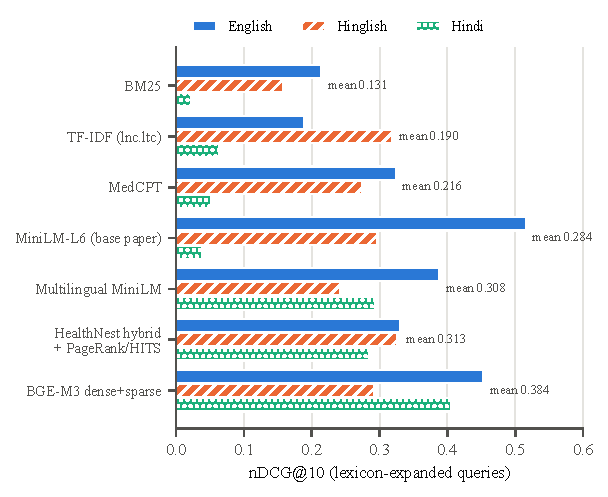
\includegraphics[width=\columnwidth]{figures/fig_ndcg_language.pdf}
  \caption{nDCG@10 by query language. The English-only model of~\cite{fedallah2026} is best in English but almost fails in Hindi; multilingual models keep Hindi usable.}
  \label{fig:lang}
\end{figure}

\begin{table}[t]
\caption{P@5, R@10 and F1@10 by language}
\label{tab:language}
\centering
\setlength{\tabcolsep}{2.2pt}
\begin{tabular}{@{}lccccccccc@{}}
\toprule
 & \multicolumn{3}{c}{English} & \multicolumn{3}{c}{Hinglish} & \multicolumn{3}{c}{Hindi} \\
\cmidrule(lr){2-4}\cmidrule(lr){5-7}\cmidrule(l){8-10}
System & P@5 & R & F1 & P@5 & R & F1 & P@5 & R & F1 \\
\midrule
MiniLM-L6 (as in \cite{fedallah2026}) & 0.605 & 0.368 & 0.342 & 0.390 & 0.205 & 0.217 & 0.050 & 0.037 & 0.030 \\
Multilingual MiniLM \cite{reimers2020} & 0.460 & 0.340 & 0.305 & 0.360 & 0.196 & 0.208 & 0.315 & 0.172 & 0.173 \\
\textbf{HealthNest} (RRF + PR/HITS) & 0.420 & 0.315 & 0.281 & 0.500 & 0.228 & 0.255 & 0.320 & 0.171 & 0.178 \\
BGE-M3 \cite{chen2024} & 0.540 & 0.330 & 0.299 & 0.410 & 0.229 & 0.234 & 0.445 & 0.221 & 0.229 \\

\bottomrule
\end{tabular}
\end{table}

\subsection{Effect of each IR component}
Fig.~\ref{fig:components} isolates the link-analysis and feedback components. Weights were tuned on the even-numbered needs and reported on the odd-numbered ones. PageRank+HITS re-ranking raised nDCG@10 from 0.316 to 0.330 in all three languages, but the gain is not significant ($p=0.11$). Pseudo-relevance feedback gave only $+0.007$ ($p=0.51$), hurt English slightly and caused two additional wrong abstentions, so it is disabled by default. Explicit feedback, simulated by marking the first five results with the relevance labels and scoring only unseen passages (the residual collection~\cite{manning2008}), raised nDCG@10 from 0.274 to 0.365 ($p<0.001$), with gains in every language.

\begin{figure}[t]
  \centering
  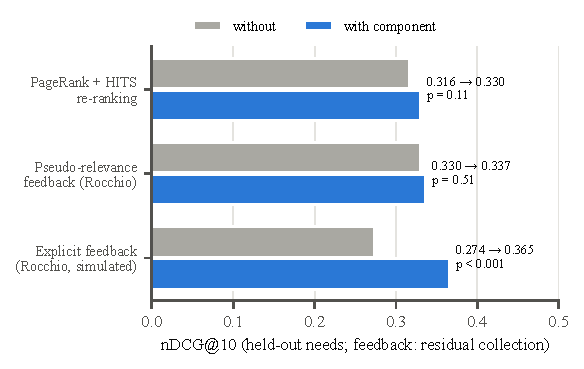
\includegraphics[width=\columnwidth]{figures/fig_components.pdf}
  \caption{Effect of link analysis and Rocchio feedback on nDCG@10.}
  \label{fig:components}
\end{figure}

\subsection{Answer or abstain}
Table~\ref{tab:abstain} evaluates the full pipeline's decision to answer. All 20 off-topic questions were refused in every language (no false positives, precision 1.000), and 39 of 40 English health questions were answered (accuracy 0.983, F1 0.987). Recall falls to 0.375 for Hinglish and 0.075 for Hindi: the concept-coverage gate requires query terms to appear in English passages, which Devanagari queries rarely satisfy, so these users are mostly offered the Wikipedia search instead.

\begin{table}[t]
\caption{Answer/abstain decision (``answer'' = positive class)}
\label{tab:abstain}
\centering
\setlength{\tabcolsep}{2.6pt}
\begin{tabular}{@{}lcccccccc@{}}
\toprule
Questions & TP & FP & FN & TN & Acc. & Prec. & Rec. & F1 \\
\midrule
English + off-topic & 39 & 0 & 1 & 20 & 0.983 & 1.000 & 0.975 & 0.987 \\
Hinglish + off-topic & 15 & 0 & 25 & 20 & 0.583 & 1.000 & 0.375 & 0.545 \\
Hindi + off-topic & 3 & 0 & 37 & 20 & 0.383 & 1.000 & 0.075 & 0.140 \\
All 140 questions & 57 & 0 & 63 & 20 & 0.550 & 1.000 & 0.475 & 0.644 \\

\bottomrule
\end{tabular}
\end{table}

\subsection{Comparison with existing work}
\textbf{Base paper~\cite{fedallah2026}.} On our data, its retriever (all-MiniLM-L6-v2) reached a mean nDCG@10 of 0.284 against 0.313 for HealthNest and 0.384 for BGE-M3. It was the strongest model for English (0.515, better than BGE-M3 by 0.063, $p=0.03$) but scored 0.038 in Hindi, confirming the multilingual limitation that its authors list as future work. Because~\cite{fedallah2026} always passes the top five chunks to the LLM without a similarity threshold, off-topic questions reach the generator and refusal depends on the prompt; HealthNest refuses them at retrieval time (20/20). The faithfulness score of 0.888 in~\cite{fedallah2026} measures generation with an LLM judge on 56 chunks and is not directly comparable to our retrieval metrics.

\textbf{MIRAGE~\cite{xiong2024}.} MIRAGE found MedCPT among the strongest retrievers for PubMed-style medical QA. On consumer questions in three languages, MedCPT ranked below every general-purpose embedding model here (nDCG@10 0.216) and almost failed in Hindi (0.051), suggesting that domain-specific retrievers trained on English literature search do not transfer to lay, multilingual questions.

\subsection{Discussion}
Dense and fused retrieval clearly beat lexical retrieval for lay questions, which rarely contain the medical term used in MedQuAD titles. The Hinglish lexicon matters more than the embedding model for Hinglish: it lifted TF-IDF from 0.150 to 0.319 nDCG@10, while no embedding model improved Hinglish significantly over the others. Link analysis helps modestly and consistently; relevance feedback helps substantially when the user supplies it, but not when it is guessed. Abstention is safe (no off-topic answer) but too conservative for Hindi and Hinglish.

%====================================================================
\section{Conclusions and Limitations}
%====================================================================
HealthNest shows that classic IR algorithms remain useful inside a modern RAG system: TF-IDF, dense retrieval and RRF provide the evidence, PageRank, HITS and topic-sensitive PageRank organise it, and Rocchio feedback lets users steer it, while citations, fact checking, abstention and verbatim handling of personal documents make answers verifiable. Compared with the base RAG architecture~\cite{fedallah2026}, it adds measured retrieval quality, refusal of off-topic questions, Hinglish and Hindi support and private document handling. A multilingual embedding model (BGE-M3) is the most promising next upgrade.

\textbf{Limitations.} (1) The 140 test questions were drafted with AI assistance and still need review by native speakers; relevance labels come from passage titles, so some relevant passages under other titles count as wrong. (2) The sample is small and $p$-values are not corrected for multiple comparisons. (3) The 0.45 dense-similarity gate was chosen on the same questions it is evaluated on. (4) Answer quality was evaluated with the offline generator; LLM answers and RAGAS faithfulness were not measured, so no direct comparison with the 0.888 of~\cite{fedallah2026} is possible. (5) The simulated relevance feedback assumes a perfect user. (6) Topic links are inferred from names in text, not real hyperlinks. (7) Scanned or handwritten prescriptions and reports cannot be read, and lab-report parsing is rule-based. (8) HealthNest is an information tool, not medical advice.

\section*{Acknowledgment}
An AI coding assistant was used during implementation and evaluation; its contributions and the team's review tasks are logged in \texttt{docs/AI\_USAGE\_LOG.md} of the project repository.

%====================================================================
% References: numbered IEEE citations; entries written in the format
% requested by the course (Author, Year, Month. Title. In Venue (pp.)).
%====================================================================
\begin{thebibliography}{00}
\bibitem{fedallah2026} Fedallah, B. and \.{I}nik, \"{O}., 2026, June. RAG-based knowledge retrieval architecture for medical web platforms. In \textit{2026 2nd International Symposium on AI-Driven Engineering Systems (ISADES)} (pp. 1--3). IEEE. doi: 10.1109/ISADES69945.2026.11608242.
\bibitem{lewis2020} Lewis, P., Perez, E., Piktus, A., Petroni, F., Karpukhin, V., Goyal, N., K\"{u}ttler, H., Lewis, M., Yih, W.T., Rockt\"{a}schel, T., Riedel, S. and Kiela, D., 2020. Retrieval-augmented generation for knowledge-intensive NLP tasks. In \textit{Advances in Neural Information Processing Systems} (Vol. 33, pp. 9459--9474).
\bibitem{es2024} Es, S., James, J., Espinosa-Anke, L. and Schockaert, S., 2024, March. RAGAS: Automated evaluation of retrieval augmented generation. In \textit{Proceedings of the 18th Conference of the European Chapter of the Association for Computational Linguistics: System Demonstrations} (pp. 150--158).
\bibitem{xiong2024} Xiong, G., Jin, Q., Lu, Z. and Zhang, A., 2024, August. Benchmarking retrieval-augmented generation for medicine. In \textit{Findings of the Association for Computational Linguistics: ACL 2024} (pp. 6233--6251).
\bibitem{abacha2019} Ben Abacha, A. and Demner-Fushman, D., 2019. A question-entailment approach to question answering. \textit{BMC Bioinformatics}, 20(1), p. 511.
\bibitem{robertson2009} Robertson, S. and Zaragoza, H., 2009. The probabilistic relevance framework: BM25 and beyond. \textit{Foundations and Trends in Information Retrieval}, 3(4), pp. 333--389.
\bibitem{manning2008} Manning, C.D., Raghavan, P. and Sch\"{u}tze, H., 2008. \textit{Introduction to Information Retrieval}. Cambridge University Press.
\bibitem{reimers2020} Reimers, N. and Gurevych, I., 2020, November. Making monolingual sentence embeddings multilingual using knowledge distillation. In \textit{Proceedings of the 2020 Conference on Empirical Methods in Natural Language Processing (EMNLP)} (pp. 4512--4525).
\bibitem{jin2023} Jin, Q., Kim, W., Chen, Q., Comeau, D.C., Yeganova, L., Wilbur, W.J. and Lu, Z., 2023. MedCPT: Contrastive pre-trained transformers with large-scale PubMed search logs for zero-shot biomedical information retrieval. \textit{Bioinformatics}, 39(11), btad651.
\bibitem{chen2024} Chen, J., Xiao, S., Zhang, P., Luo, K., Lian, D. and Liu, Z., 2024, August. M3-Embedding: Multi-linguality, multi-functionality, multi-granularity text embeddings through self-knowledge distillation. In \textit{Findings of the Association for Computational Linguistics: ACL 2024} (pp. 2318--2335).
\bibitem{cormack2009} Cormack, G.V., Clarke, C.L.A. and B\"{u}ttcher, S., 2009, July. Reciprocal rank fusion outperforms Condorcet and individual rank learning methods. In \textit{Proceedings of the 32nd International ACM SIGIR Conference on Research and Development in Information Retrieval} (pp. 758--759).
\bibitem{page1999} Page, L., Brin, S., Motwani, R. and Winograd, T., 1999. The PageRank citation ranking: Bringing order to the web. Technical Report, Stanford InfoLab.
\bibitem{kleinberg1999} Kleinberg, J.M., 1999. Authoritative sources in a hyperlinked environment. \textit{Journal of the ACM}, 46(5), pp. 604--632.
\bibitem{haveliwala2002} Haveliwala, T.H., 2002, May. Topic-sensitive PageRank. In \textit{Proceedings of the 11th International Conference on World Wide Web} (pp. 517--526).
\bibitem{rocchio1971} Rocchio, J.J., 1971. Relevance feedback in information retrieval. In G. Salton (Ed.), \textit{The SMART Retrieval System: Experiments in Automatic Document Processing} (pp. 313--323). Prentice-Hall.
\end{thebibliography}

\end{document}
